\DocumentMetadata{tagging=on}
\documentclass{article}
\ifdefined\Uchar
  \usepackage{lua-unicode-math}
\fi
\usepackage{tikz}
\usetikzlibrary{tikzmark,decorations.pathreplacing}

\title{tikzmark tagging test}

\begin{document}

\tikzset{tikzmark prefix=ex1-}
\[
\tikzmark{a} e^{i \pi/2} = i
\]
This\tikz[remember picture,overlay,baseline=0pt] \draw[->] (0,1em)
to[bend left] ([shift={(-1ex,1ex)}]pic cs:a); is an important
equation.

\tikzset{tikzmark prefix=ex2-}
\begin{itemize}
\item A first item,\tikzmark{b}
\item A second item,\tikzmark{c}
\item A third item.\tikzmark{d}
\end{itemize}
\begin{tikzpicture}[remember picture,overlay]
\draw[decorate,decoration={brace}] ({pic cs:c} |- {pic cs:b})
+(0,1em) -- node[right,inner sep=1em] {some items} ({pic cs:c}
|- {pic cs:d});
\end{tikzpicture}

\tikzset{tikzmark prefix=ex3-}
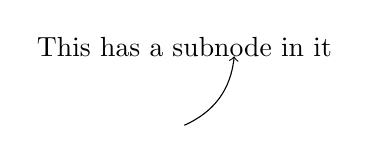
\begin{tikzpicture}[remember picture]
\node (a) at (0,0) {This has a \subnode{sub}{subnode} in it};
\draw[->] (0,-1) to[bend right] (sub);
\end{tikzpicture}

\tikzset{tikzmark prefix=ex4-}

\begin{tikzpicture}[remember picture,overlay]
\draw[->,line width=1mm,cyan] (pic cs:a) to[bend left] (pic cs:b);
\end{tikzpicture}
By placing the \tikzmark{a}code before the marks, the arrow goes
under the subsequent text and picture.

\begin{tikzpicture}
\filldraw[fill=gray] (0,0) circle[radius=1cm];
\tikzmark{b}{(-1,-1)}
\end{tikzpicture}

\tikzset{tikzmark prefix=ex5-}
Putting a node around \tikzmarknode{txt}{some text} means we can
connect text together, including in maths:
\[
\tikzmarknode{a}{\sum_{k=1}^n} k^{\tikzmarknode{b}{2}}
\]
\begin{tikzpicture}[remember picture,overlay]
\draw[->] (txt) -- (a);
\draw[->] (a.south) to[out=-90,in=-45] (b.south east);
\end{tikzpicture}

\end{document}